\chapter{Results}


%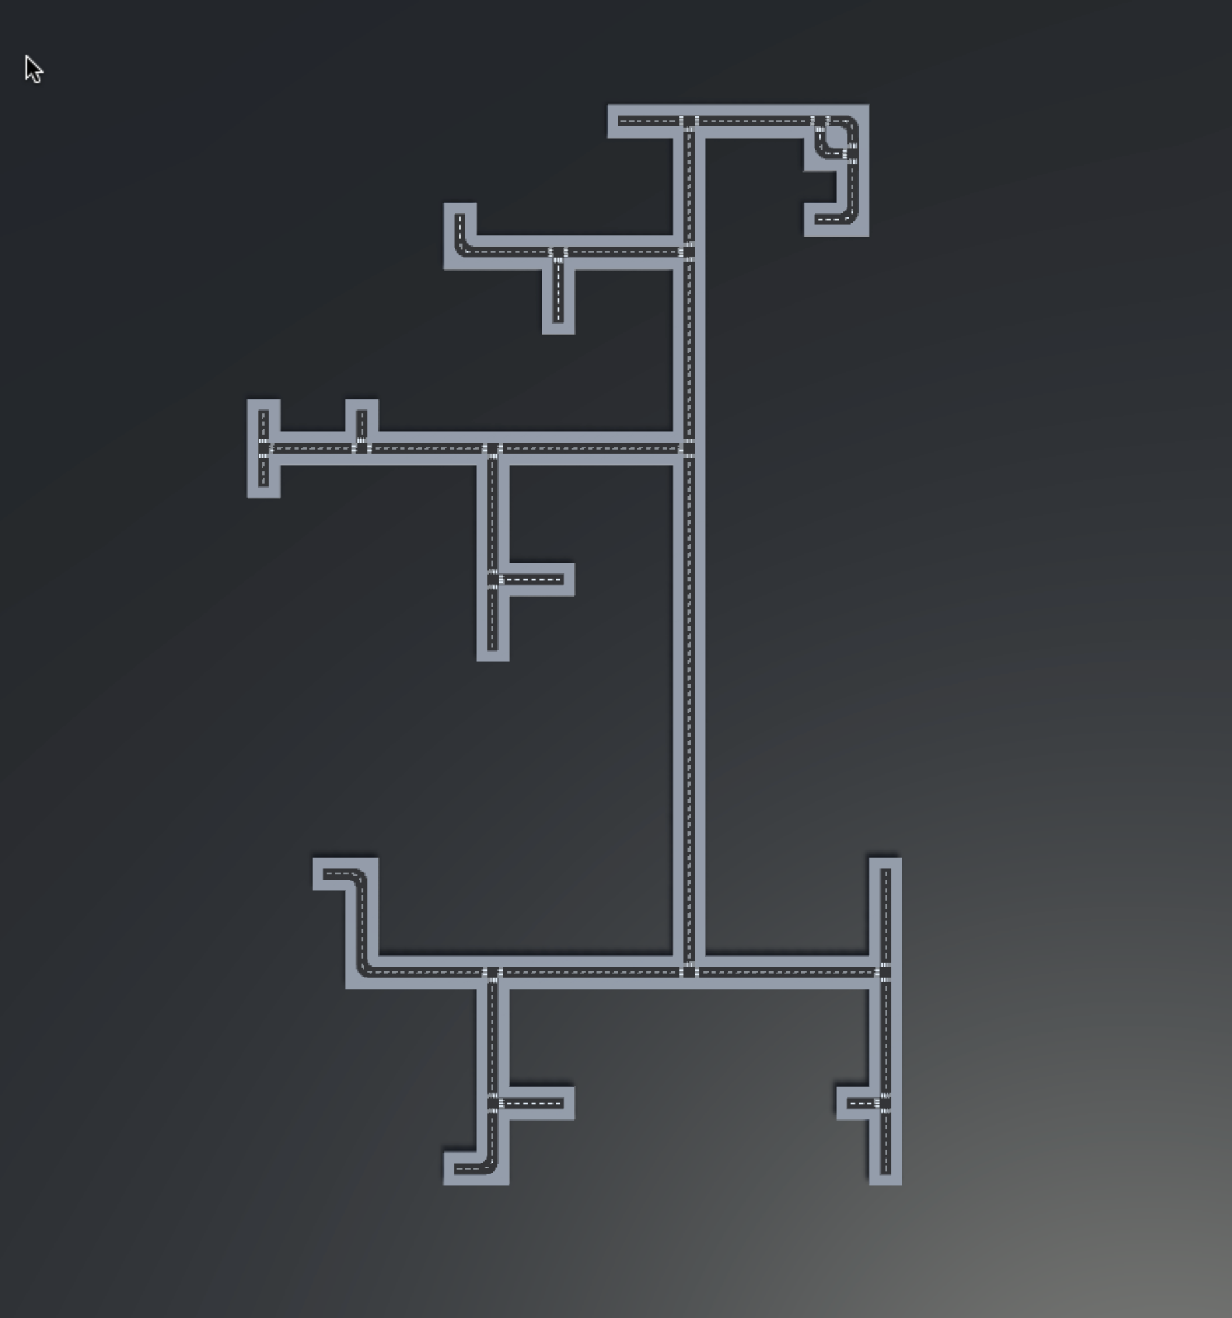
\includegraphics[scale=0.3]{5. results/Road Outpu.png}

There are several ways to plot a function of two variables, depending on the information you are interested in. For instance, if you want to see the mesh of a function so it easier to see the derivative you can use a plot like the one on the left.

\begin{figure}[h]
\caption{Example of a parametric plot ($\sin (x), \cos(x), x$)}
\vspace{0.3cm}
\centering
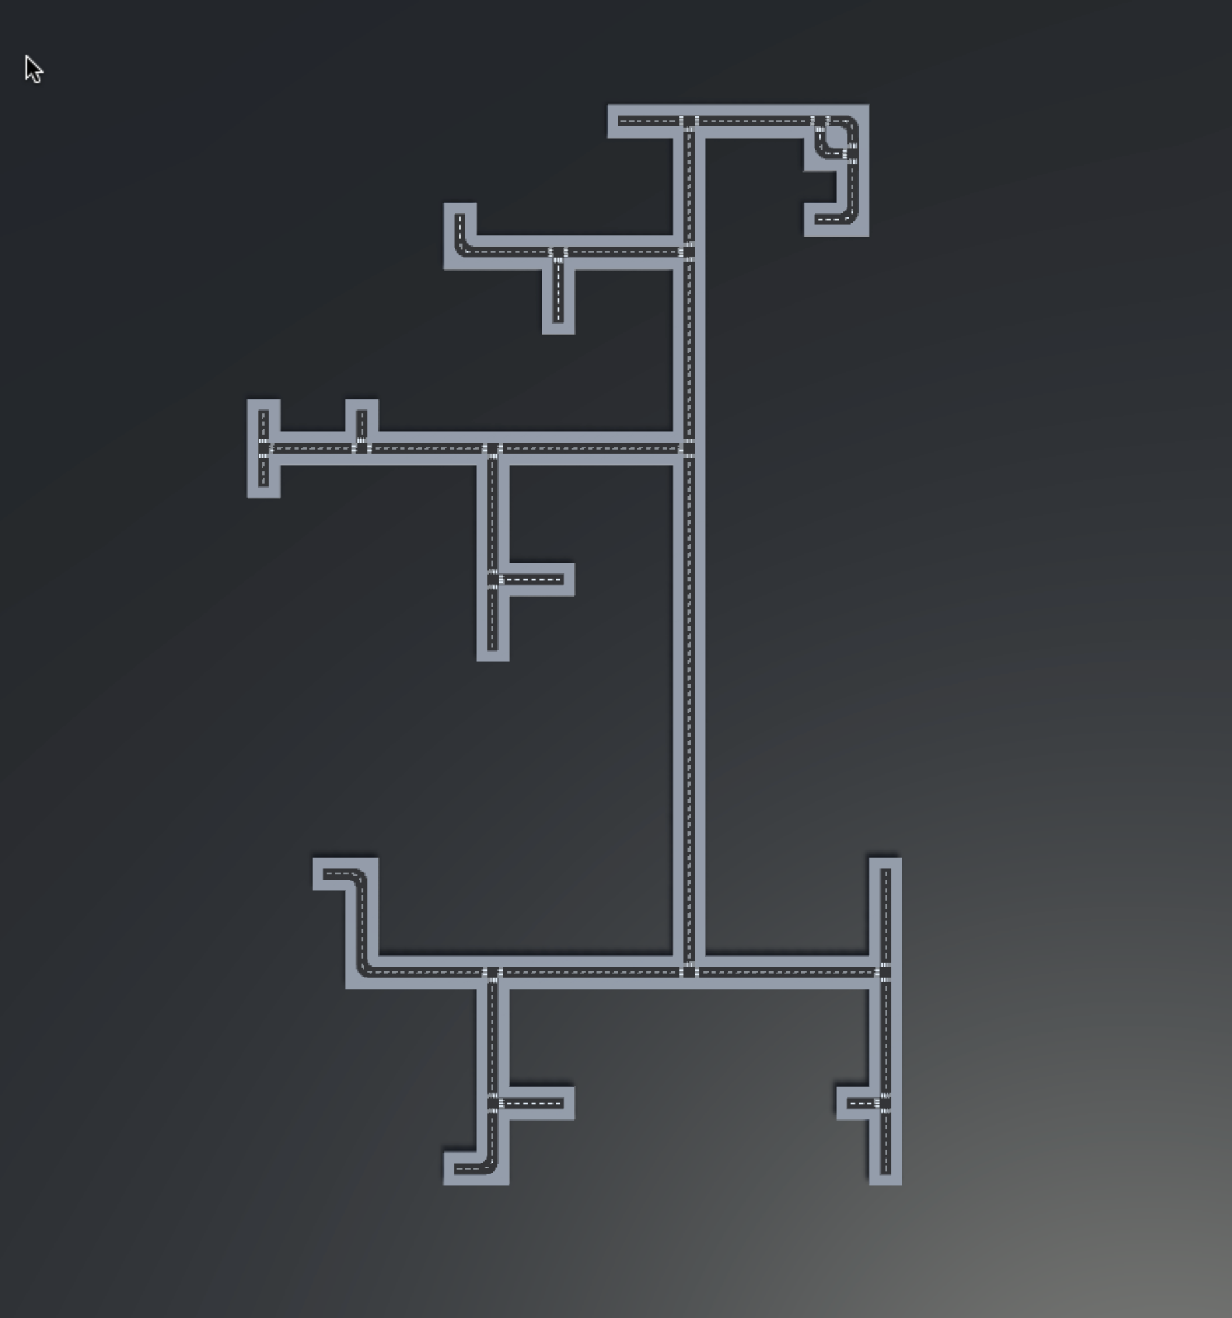
\includegraphics[width=0.6\textwidth]{5. results/Road Outpu.png}
\end{figure}

\begin{comment}

\vspace{0.5cm}

\begin{wrapfigure}{r}{0.25\textwidth} %this figure will be at the right
    \centering
    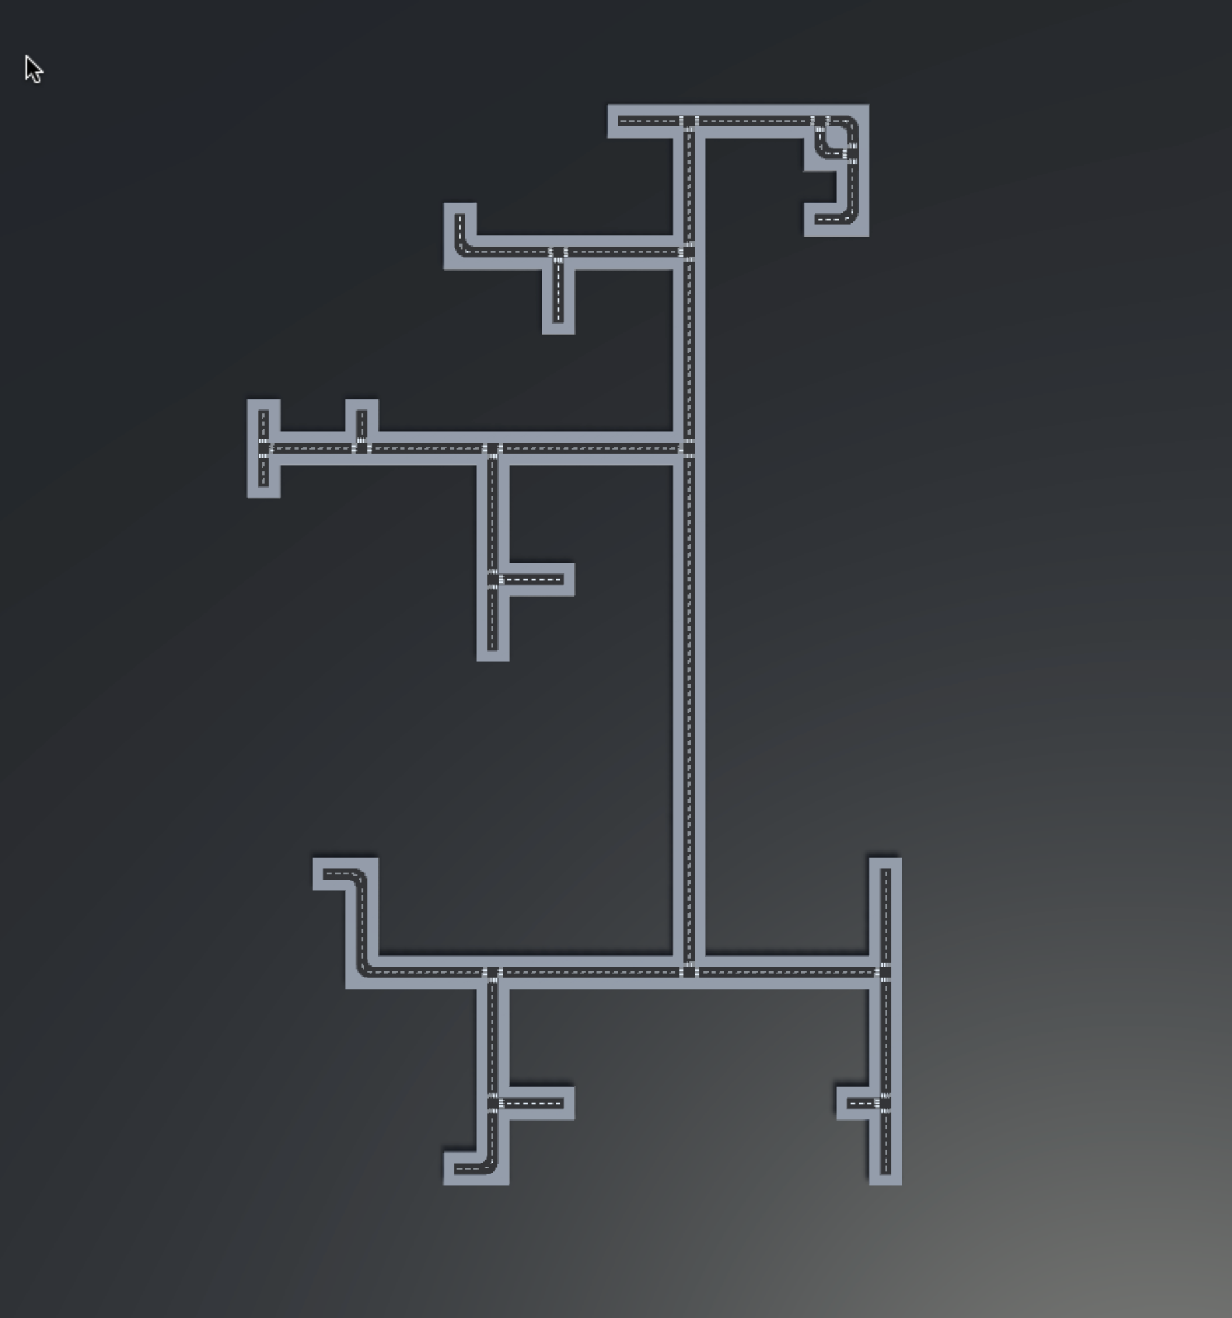
\includegraphics[width=0.25\textwidth]{5. results/Road Outpu.png}
\end{wrapfigure}

There are several ways to plot a function of two variables, depending on the information you are interested in. For instance, if you want to see the mesh of a function so it easier to see the derivative you can use a plot like the one on the left.

There are several ways to plot a function of two variables, depending on the information you are interested in. For instance, if you want to see the mesh of a function so it easier to see the derivative you can use a plot like the one on the left.

There are several ways to plot a function of two variables, depending on the information you are interested in. For instance, if you want to see the mesh of a function so it easier to see the derivative you can use a plot like the one on the left.

There are several ways to plot a function of two variables, depending on the information you are interested in. For instance, if you want to see the mesh of a function so it easier to see the derivative you can use a plot like the one on the left.

\begin{SCfigure}[0.5][h]
\caption{Using again the picture of the universe. 
         This caption will be on the right}
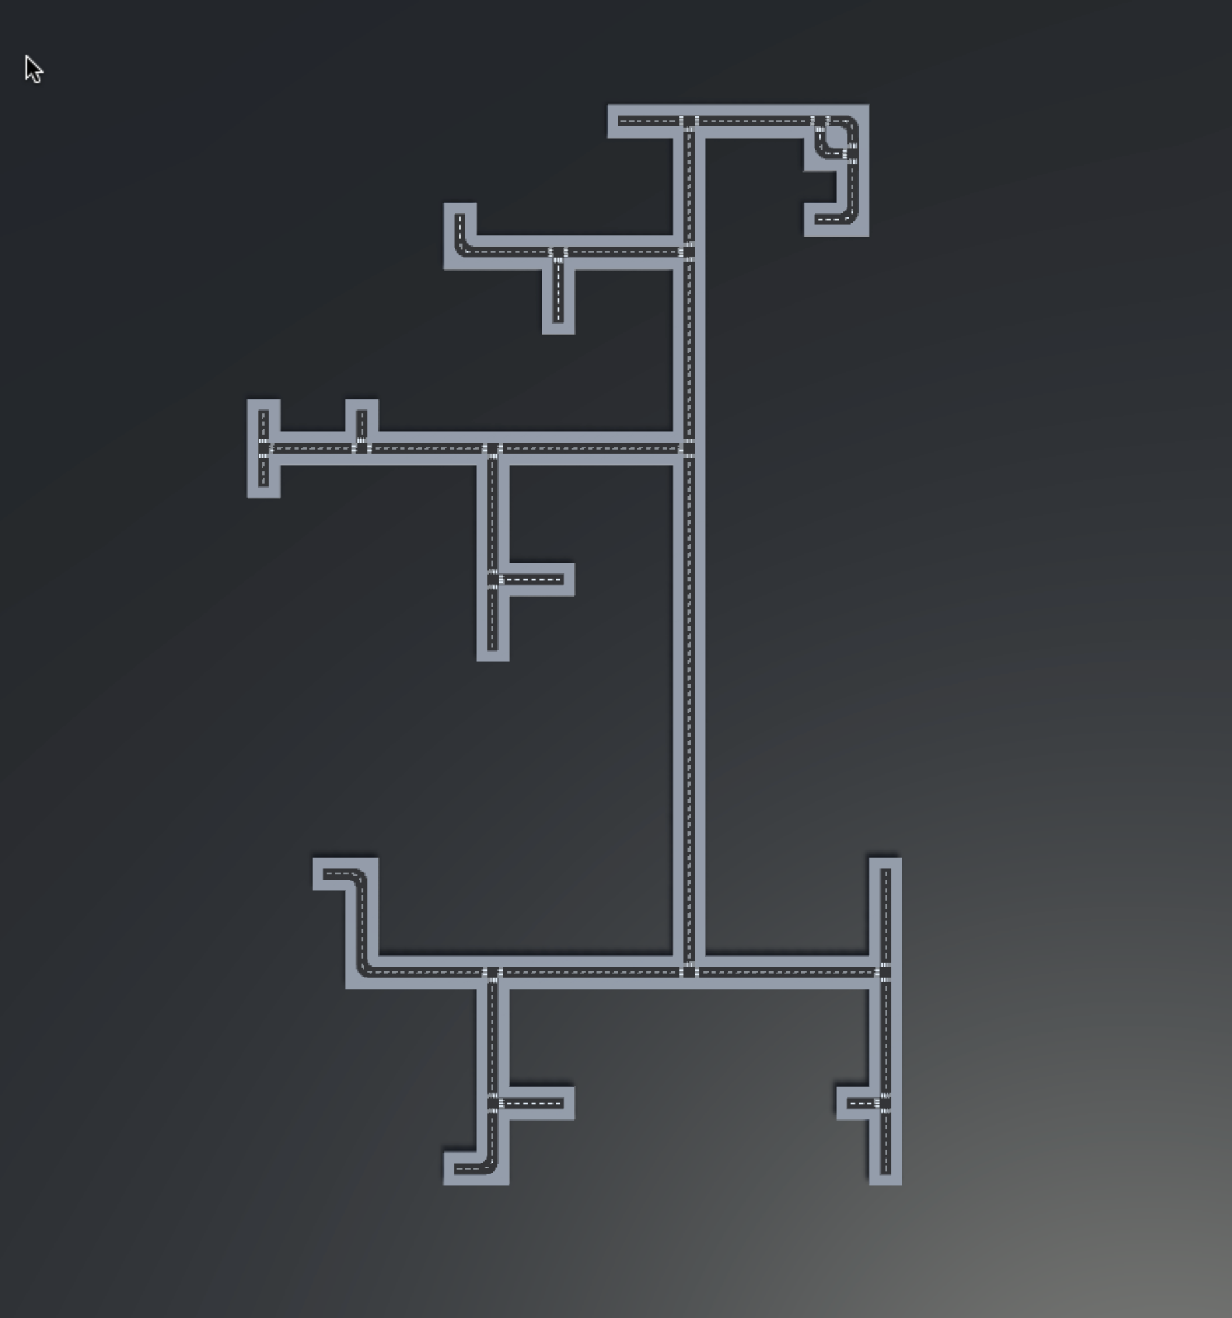
\includegraphics[width=0.6\textwidth]{5. results/Road Outpu.png}
\end{SCfigure}
\end{comment}